\documentclass[conference]{IEEEtran}
\IEEEoverridecommandlockouts

% Packages
\usepackage{amsmath,amssymb}
\usepackage{graphicx}
\usepackage{tikz}
\usetikzlibrary{positioning,arrows.meta}
\usepackage{hyperref}
\usepackage{cite}

\begin{document}

% Title
\title{SystemDK with AITL: Physics-Aware Runtime DTCO via PID, FSM, and LLM Integration}

\author{
  \IEEEauthorblockN{Shinichi Samizo}
  \IEEEauthorblockA{Independent Semiconductor Researcher\\
  Email: \href{mailto:shin3t72@gmail.com}{shin3t72@gmail.com}}
}

\maketitle

% Abstract
\begin{abstract}
This paper presents SystemDK with AITL, a framework that extends conventional Design-Technology Co-Optimization (DTCO) by embedding control-theoretic loops directly into EDA flows. Compact PID controllers and FSM supervisors stabilize runtime variations caused by interconnect RC delay, thermal coupling, stress-induced threshold shifts, and EMI/EMC disturbances. Future extensions (AITL Next) integrate lightweight LLM analyzers for adaptive PID retuning and FSM rule regeneration. The framework incorporates FEM analysis and S-parameter measurements into synthesis, P\&R, and STA, ensuring physics-aware closure. Simulations demonstrate order-of-magnitude improvements in timing stability, thermal robustness, and jitter suppression.
\end{abstract}

\begin{IEEEkeywords}
DTCO, CFET, PID control, FSM, LLM, EMI/EMC, thermal management, timing jitter, EDA.
\end{IEEEkeywords}

% Introduction
\section{Introduction}
Scaling to sub-2nm nodes and CFET integration introduces critical runtime effects:
\begin{itemize}
  \item RC delay variation due to interconnect scaling and BEOL resistance growth,
  \item vertical thermal coupling in 3D-ICs,
  \item stress-induced $V_{th}$ shifts around TSVs and CFET stacks,
  \item EMI/EMC noise degrading jitter and link reliability.
\end{itemize}
Traditional DTCO applies static guardbands, leading to inefficiency. SystemDK with AITL proposes embedding compact control (PID + FSM) in the loop, and in the next step, LLM-based adaptation.

% Proposed Framework
\section{Proposed Framework}
\subsection{AITL Base}
A compact PID compensates delay/thermal/voltage variations, while an FSM supervises modes and safety thresholds. Physics telemetry (delay, temperature, jitter) feeds the controllers; compact models map measured quantities to actionable constraints for EDA.

\subsection{AITL Next}
A lightweight LLM analyzes EDA/telemetry logs, recommends new gains $(K_p, K_i, K_d)$, and regenerates FSM rules when operating points drift (aging, workload, ambient). This enables adaptive retuning without human-in-the-loop during field operation.

% Figure 1: TikZ diagram
\begin{figure*}[t]
\centering
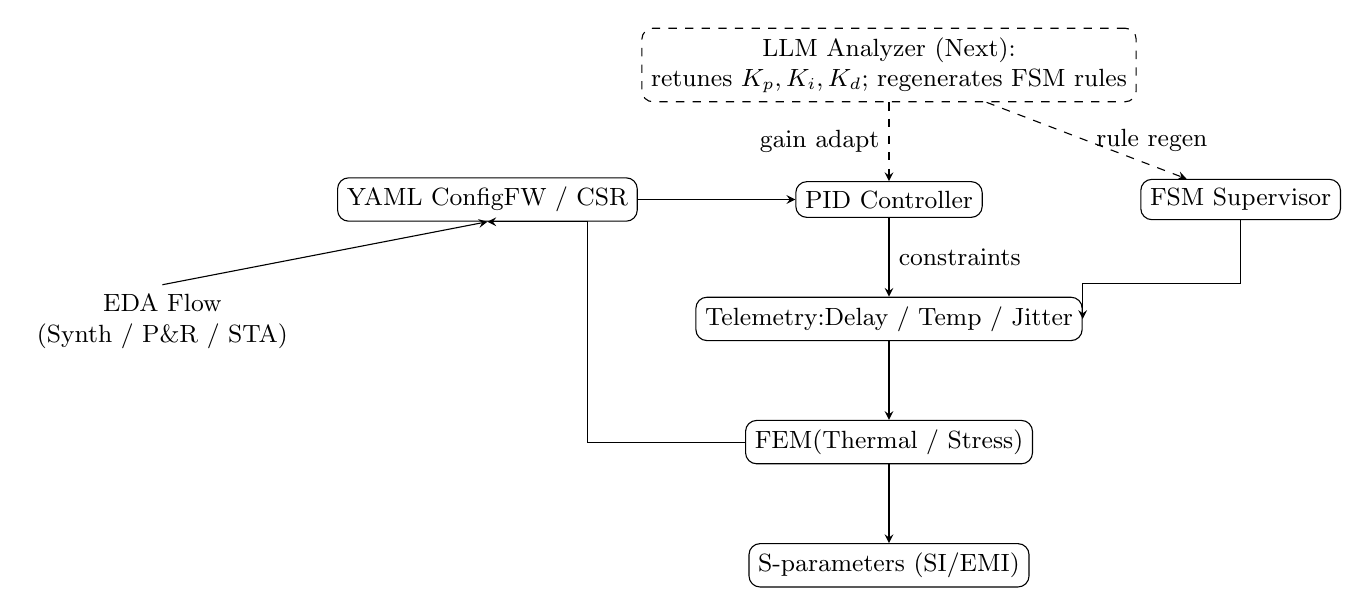
\begin{tikzpicture}[node distance=10mm and 20mm, >=stealth, font=\small]

% Nodes
\node[draw, rectangle, rounded corners] (yaml) {YAML Config\\FW / CSR};
\node[draw, rectangle, rounded corners, right=of yaml] (pid) {PID Controller};
\node[draw, rectangle, rounded corners, right=of pid] (fsm) {FSM Supervisor};

\node[draw, rectangle, rounded corners, below=of pid] (tele) {Telemetry:\\Delay / Temp / Jitter};
\node[draw, rectangle, rounded corners, below=of tele] (fem) {FEM\\(Thermal / Stress)};
\node[draw, rectangle, rounded corners, below=of fem] (sparam) {S-parameters (SI/EMI)};

\node[draw, rectangle, dashed, rounded corners, above=of pid, align=center] (llm) {LLM Analyzer (Next):\\retunes $K_p,K_i,K_d$; regenerates FSM rules};

% Arrows
\draw[->] (yaml) -- (pid);
\draw[->] (pid) -- (tele) node[midway,right] {constraints};
\draw[->] (tele) -- (fem);
\draw[->] (fem) -- (sparam);
\draw[->] (fem.west) -| ++(-2,0) |- (yaml.south); % FEM → EDA Flow

\node[below left=8mm and 5mm of yaml, align=center] (eda) {EDA Flow\\(Synth / P\&R / STA)};
\draw[->] (eda.north) -- (yaml.south);

\draw[->, dashed] (llm) -- (pid) node[midway,left] {gain adapt};
\draw[->, dashed] (llm) -- (fsm) node[midway,right] {rule regen};

\draw[->] (fsm.south) |- ++(0,-0.8) -| (tele.east); % rerouted arrow

\end{tikzpicture}
\caption{System overview (two-column): runtime telemetry → compact physics models → PID/FSM runtime control → actuators, with EDA sign-off integration; an optional LLM (Next) provides adaptive gain retuning and FSM rule regeneration. Arrows are rerouted to avoid block overlap.}
\label{fig:overview}
\end{figure*}

% Analytical Models
\section{Analytical Models and EDA Mapping}
\subsection{RC Delay Model}
We model the path delay with temperature $T$, stress $\sigma$, and frequency $f$ dependence:
\begin{equation}
t_{pd}(T,\sigma,f) = R_0(1+\alpha_T(T-T_0)+\alpha_\sigma\sigma)C(f)+\Delta_{EMI}(f).
\end{equation}
Mapped to STA path-delay constraints.

\subsection{Thermal Coupling}
A lumped die model gives
\begin{equation}
C_{th}\frac{dT}{dt} + \frac{T-T_{amb}}{R_{th}} = P_{chip}(t),
\end{equation}
which we translate into P\&R thermal placement limits.

\subsection{Stress-Induced $V_{th}$ Shift}
A first-order model $\Delta V_{th}(\sigma) = \kappa \cdot \sigma$ is used to bound timing degradation near TSVs/CFET fins.

\subsection{EMI Injection}
Injected EMI is represented as
\begin{equation}
v_{emi}(t) = A\sin(2\pi f_{emi}t),
\end{equation}
mapped to SI/EMI jitter constraints.

% Simulation Results
\section{Simulation Results with EDA Implications}
\subsection{RC Delay Compensation}
\includegraphics[width=0.48\textwidth]{figs/sim_delay_rc.png}
\caption{RC delay variation normalized (Uncontrolled, PID, PID+FSM).}

\subsection{Thermal Response Control}
\includegraphics[width=0.48\textwidth]{figs/sim_thermal_response.png}
\caption{Thermal response $\Delta T$ reduction with PID and PID+FSM.}

\subsection{EMI Jitter Suppression}
\includegraphics[width=0.48\textwidth]{figs/sim_emi_jitter.png}
\caption{Jitter reduction under injected EMI.}

\subsection{FEM Analysis}
\includegraphics[width=0.48\textwidth]{figs/fem_thermal_map.png}
\includegraphics[width=0.48\textwidth]{figs/fem_stress_map.png}
\caption{FEM maps: thermal hotspot (top) and TSV-induced stress (bottom).}

\subsection{S-Parameter Analysis}
\includegraphics[width=0.48\textwidth]{figs/sparam_s11s21.png}
\caption{$S_{11}/S_{21}$ measurements validate SI/EMI resilience with control.}

% Implementation
\section{Implementation PoC}
We implemented a synthesizable PID, FSM transitions, and YAML-driven configuration in Verilog; CSRs are exposed over APB/AXI-Lite. Telemetry hooks connect to on-die sensors and firmware. The PoC integrates with synthesis, P\&R, and STA to demonstrate closed-loop DTCO.

% Discussion
\section{Discussion}
\textbf{Guardbands → adaptive loops:} Static margins are replaced by feedback that reacts to measured physics.  
\textbf{Static sign-off → dynamic runtime closure:} Sign-off artifacts (FEM, SI) become runtime constraints.  
\textbf{Reliability:} Cross-domain resilience (delay, thermal, stress, EMI) improves lifetime and QoR.

% Conclusion
\section{Conclusion and Future Work}
AITL Base (PID+FSM) establishes runtime stabilization with measurable benefits on timing, thermal, and jitter metrics. AITL Next will integrate a lightweight LLM to analyze logs, retune gains, and regenerate FSM rules online. We target prototype chips, collaboration with EDA tools, and AI-driven DTCO.

% References
\bibliographystyle{IEEEtran}
\bibliography{refs}

% Author Bio
\section*{Author Biography}
\noindent\textbf{Shinichi Samizo} received the M.S. degree in Electrical and Electronic Engineering from Shinshu University, Japan. He worked at Seiko Epson Corporation as an engineer in semiconductor memory and mixed-signal device development, and contributed to inkjet MEMS actuators and PrecisionCore printhead technology. He is currently an independent semiconductor researcher focusing on process/device education, memory architecture, and AI system integration.\\[2pt]
\textbf{Contact:} \href{mailto:shin3t72@gmail.com}{shin3t72@gmail.com}, \href{https://github.com/Samizo-AITL}{Samizo-AITL}

\end{document}
